\chapter{Estudo de Caso}
\label{cap-case-study}

%

Neste capítulo será apresentada a utilização dos Cenários de Decisões em projetos reais, com o principal objetivo de demonstrar a reprodução de cenários em ambientes de tomada de decisão. Assim, este Capítulo é destinado ao Estudo de Caso de utilização das ferramentas Mezuro e DWing para observação de Cenários de Decisões em projetos de software.

Para tanto, será apresentada a avaliação de três projetos de softwares livres em C++. Além disso, iremos explicar os passos necessários para reproduzir a estrutura de cenários nos dois ambientes de tomadas de decisões abordados nesta monografia. Assim, será apresentado as principais evoluções e adaptação de cada ferramenta e os detalhes específicos da observação de cada cenário.

O método de execução desses estudos de casos é apresentado na Figura~\ref{method}. Nesta figura são descritos os passos necessários para reproduzir cenários em ferramentas que apoiam a tomada de decisões baseados em métricas de software que, no contexto desta monografia, consiste no Mezuro e DWing.

\graphicspath{{figuras/}}
\begin{figure}[h]
\centering
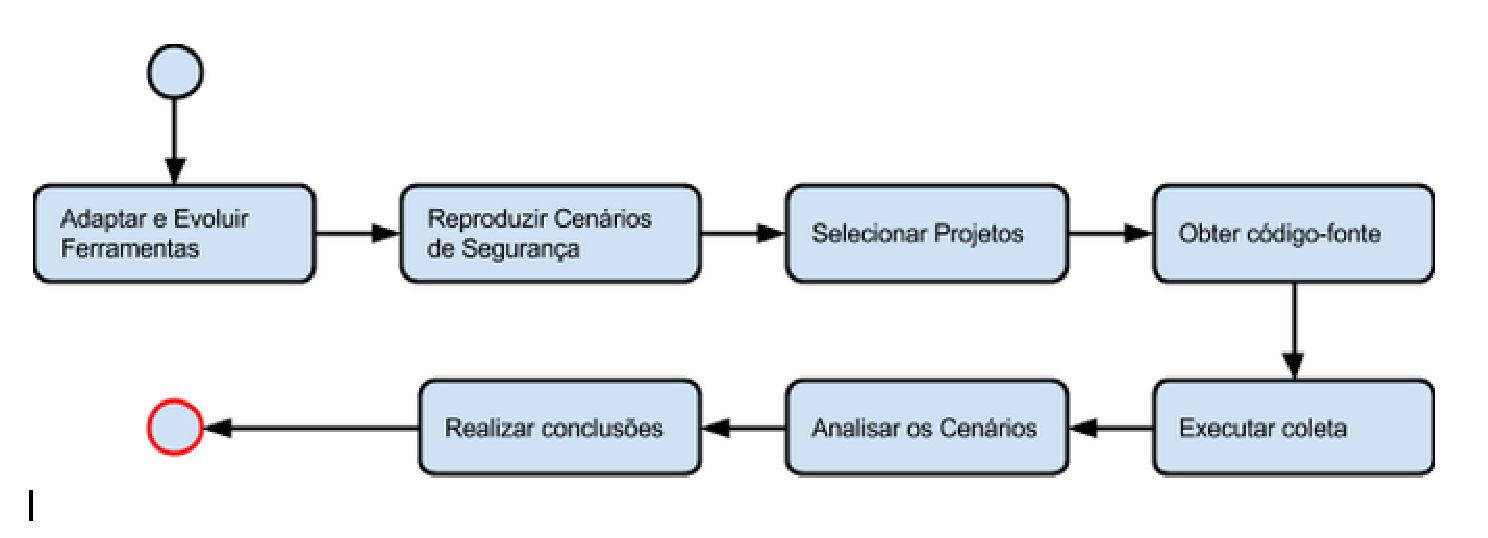
\includegraphics[width=1.0\textwidth]{fluxograma}
\caption{Método para execução dos estudos de casos.}
\label{method}
\end{figure}

Os passos da Figura~\ref{method} são melhor descritos a seguir:

\begin{enumerate}
\item \textbf{Adaptar e Evoluir Ferramentas} - Este passo consiste em evoluir as estruturas, modelos, componentes e camada de apresentação das ferramentas que serão utilizadas com o objetivo de melhor suportar a utilização de Cenários de Decisão.
\item \textbf{Reproduzir Cenários} - Uma vez que as ferramentas utilizadas já suportam a reprodução de Cenários, deve-se utilizar dessa estrutura para definir cenários reais para avaliação de projetos de software. No contexto dessa monografia, esse passo consiste em reproduzir os Cenários de Segurança criados no Mezuro e no DWing.
\item \textbf{Selecionar Projetos} - Esta etapa consiste em definir quais projetos serão avaliados a partir dos cenários definidos e pode ser executada independente das ferramentas de tomada de decisão, variando de acordo com os objetivos de utilização dos Cenários.
\item \textbf{Obter Código-Fonte} - Uma vez selecionados os projetos, o próximo passo é obter o código-fonte referente aos projetos escolhidos. Algumas ferramentas. como o Mezuro, já possuem bom suporte para automatizar esse passo.
\item \textbf{Executar Coleta} - Esta etapa consiste na obtenção dos valores de métricas dos códigos-fontes dos projetos selecionados que deve ser automatizado. A saída desta etapa deverá ser processada pelas ferramentas trabalhadas para proporcionar a análise dos projetos. O esforço nessa etapa deve-se reduzir a coletar somente as métricas necessárias para composição dos Cenários de Decisão utilizados.
\item \textbf{Analisar Cenários} - A partir dos resultados obtidos, deve-se utilizar os Cenários de Decisão para observar as características do estado atual do projeto analisado. No contexto desse trabalho, esta etapa consiste em analisar quais os principais módulos oferecem riscos de segurança ao software.
\item \textbf{Realizar Conclusões} - Esta etapa final consiste em realizar ações a partir da compreensão dos Cenários observados, seja para fins de estudos ou para fins de desenvolvimento do software. 
\end{enumerate}


Estes passos metodológicos devem ser reproduzidos para cada ferramenta utilizada, sendo que uma vez que uma ferramenta já suporta adequadamente a observação de Cenários de Decisão, os passos 1 e 2 não precisam ser repetidos para análise de novos projetos.


\section{Criação dos Cenários do Mezuro}
\label{mezuro-cenarios}

explicar primeiro como o Mezuro foi utilizado para suportar os Cenários, o que foi adaptado e melhorado para melhor suportar cenários, etc.

Depois deve-se mostrar a estrutura de cada cenário dentro da ferramenta (scripts e configuração)

\section{Criação dos Cenários do DWing}
\label{dw-cenarios}

explicar primeiro como o DW foi utilizado para suportar os Cenários, o que foi adaptado e melhorado para melhor suportar cenários, etc.

Depois deve-se mostrar a estrutura de cada cenário dentro da ferramenta (scripts e configuração)

\section{Projetos analisados}
\label{cap-projects}

Nesta monografia definimos a técnica de Cenários de Decisão e propomos um conjunto de cenários para tomada de decisão sobre a segurança do software, seja a partir da utilização de métricas de \emph{design} ou através de métricas de vulnerabilidades. Para apresentar como estes cenários podem ser utilizados, foram analisados três softwares livres. 

Como discutido no Seção \ref{cap-cenarios-sec-definicaocenarios} do Capítulo de Cenários, nos restringimos a apenas projetos escritos em C++. A seguir é feita uma pequena introdução à cada um dos projetos escolhidos.

\subsection{GNU Octave}
\label{section-octave}

O GNU Octave é um projeto desenvolvido em C++ que consiste em uma linguagem interpretada de alto nível destinada à computação matemática distribuída através da licença GNU General Public License \footnote{\url{http://www.gnu.org/copyleft/gpl.html}}. Ele possui uma interface baseada em linha de comando para a solução de problemas matemáticas lineares e não lineares, assim como possibilita a execução de experimentos numéricos. Além disso, também provê um conjunto extensivo de ferramentas para geração de gráficos, visualização e manipulação de dados.

Outras informações específicas sobre o projeto GNU Octave podem ser obtidas através da documentação oficial do projeto, disponível na página \url{https://www.gnu.org/software/octave/}.

O código fonte do projeto está disponível na página \url{ftp://ftp.gnu.org/gnu/octave}. Lá, além da versão atual, podemos ter acesso ao código de releases anteriores.

Este projeto será analisado tanto através do Mezuro quanto através do DWing.


==== MOSTRAR OS CENÀRIOS EM CADA FERRAMENTA ====


\subsection{Projeto 2}
\label{}

Projeto a ser analisado somente através do Mezuro

\subsection{Projeto 3}
\label{}

Projeto a ser analisado somente através do DWing


\section{Coleta de Dados}

O Mezuro já trabalha em conjunto com o Analizo\footnote{\url{http://www.analizo.org/}}. O Analizo é uma ferramenta de análise estática de código e dá suporte a diversas métricas, inclusive as métricas discutidas no cápitulo 2, tanto de \emph{design} quanto de vulnerabilidade. Um ambiente de DW não está atrelado a apenas uma fonte de dados, podendo utilizar diversas fontes. Dessa forma, utilizamos o Analizo para coletar as métricas e gerar o insumo para a análise dos cenários em ambas as ferramentas.

Porém, identificamos um problema com o Analizo em relação as coleta de métricas de vulnerabilidade. Para projetos pequenos e simples as métricas de vulnerabilidade podem ser coletadas.  Contudo, para projetos maiores e mais complexos, com arquitetura bem definida, o Analizo não consegue gerar tais métricas. Isso se deve ao fato do Analizo utilizar o \emph{Clang Static Analizer}\footnote{\url{http://clang-analyzer.llvm.org/}}, que é outra ferramenta livre que faz análise estática para identificação de bugs em projetos C/C++, para a geração das métricas de vulnerabilidade. A utilização do \emph{clang} consiste em chamar o comando \emph{scan-build}  e o comando de compilação do programa, por exemplo \emph{\"scan-build gcc myprog.c\"}. Foi verificado que o Analizo chama o \emph{clang} em seu código para cada arquivo, usando apenas o comando \emph{gcc} em cada um deles. Isso pode funcionar para projetos simples, porém projetos mais complexos são compilados geralmente com \emph{\"Makefile\"}, com diversas linhas de compilação. Não consguindo compilar o código, o \emph{clang} não consegue executar, fazendo com que o Analizo, por sua vez, não consiga extrair as métricas de vulnerabilidade. 

Grandes alterações deveriam ser feitas para fazer com que o Analizo pudesse gerar os valores dessas métricas para projetos grantes, não cabendo ao escopo e tempo desta monografia. Esse problema afeta diretamente ao Mezuro, pois, dependente do relatório gerado pelo Analizo, não consegue os valores de métricas de vulnerabilidade para projetos maiores. Como o ambiente de DWing pode ter diversas fontes de dados, podemos recorrer a outra fonte de dados que ofereça apenas as métricas de segurança.

Dessa forma, decidimos em usar o \emph{clang} para extrair as métricas de vulnerabilidade. O \emph{clang} gera um relatório no formato HTML. Foi feito um parser para transformar o HTML em um arquivo CSV, com a mesma estrutura fornecida pelo Analizo. Assim, o ambiente de DWing pode utilizar desse arquivo CSV gerado pelo parser para se alimentar das métricas de vulnerabildade da mesma maneira que trata o CSV gerado pelo próŕio Analizo. O parser foi desenvolvido na linguagem perl justamente para aproveitarmos das lógicas de programação e códigos do próprio Analizo.

======== EXPLICAR COMO O MEZURO UTILIZA OS DADOS do Analizo, Como funciona a Integração(brevemente)=====


======== EXPLICAR BREVEMENTE ETL DW =====



\section{Análise dos Cenários nas Ferramentas}

Nesta seção será apresentada Aqui, mostrar os cenários nos projetos, como podem ser visualizados, etc


\section{Conclusões}

Descrever as conclusoes obtidas com a execução do estudo de caso